%!TEX root = ../report.tex
\documentclass[report.tex]{subfiles}
\begin{document}
    \chapter{Related Works}

    % Divide the sections into Early, Late, Mid/Feature and Tightly-Coupled fusion methods
    \section{Adverse Weather Conditions Influence on Sensors}

    % \begin{itemize}

    %     \item In the realm of autonomous robots, particularly self-driving vehicles and autonomous drones, object detection has emerged as a critical computer vision problem. These applications demand accurate 2D or 3D bounding boxes for objects in complex real-world scenarios, which often include cluttered scenes, unpredictable lighting, and adverse weather conditions. To address these challenges, the most promising autonomous vehicle systems rely on input from redundant sensor modalities, as documented by several recent studies \cite{caesar2020nuscenes, Sun_2020_CVPR, ziegler2014making}. These sensor modalities include cameras, LiDAR, radar, and emerging sensors like far-infrared (FIR) and near-infrared (NIR) sensors, which hold great potential for enabling reliable object detection in adverse environments \cite{bijelic2020seeing}.

    %     \item For a typical perception system, the most common sensor is camera, and it's actually the one element that is absolutely not replaceable in autonomous driving systems. But it's also one of the most vulnerable sensors to adverse weather conditions. A camera in rain, regardless of however high resolution, can be easily incapacitated by a single water drop on the emitter or lens \cite{mardirosian2021LiDAR} as shown in the Figure \ref{fig:camera_in_rain}. Heavy snow or hail could fluctuate the image intensity and obscure the edges of the pattern of a certain object in the image or video which leads to detection failure \cite{zang2019impact}. A particular weather phenomenon, strong light, directly from the sun or artificial light source like light pollution from a skyscraper may also cause severe trouble to cameras \cite{acarballo2020libre}.
    %         \begin{figure}[h]
    %                 \centering
    %                 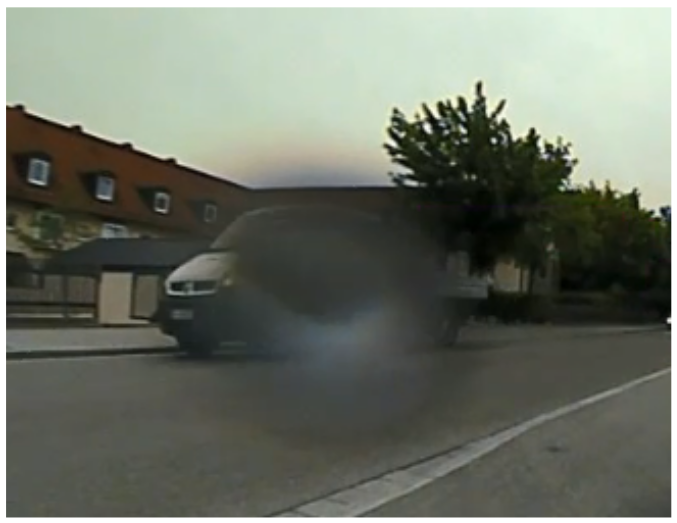
\includegraphics[width=0.5\textwidth]{images/rain_droplet.png}
    %                 \caption{Van occluded by a water droplet on the lens \cite{Nobis2020May}}
    %                 \label{fig:camera_in_rain}
    %         \end{figure}

    %     \item LiDAR is the second most commonly used sensor in autonomous driving systems. Fersch et al. \cite{fersch2016influence} suggest that for moderate levels of rainfall, LiDAR sensors with small apertures are not significantly affected. However, heavy and non-uniform precipitation rates can create clusters of fog that can lead to erroneous obstacle detection by the LiDARs. Hasirlioglu et al. \cite{hasirlioglu2016modeling} demonstrated that a rainfall rate exceeding 40 mm/hr leads to a significant drop in signal reflection intensity. Dense fog and smoke, as well as strong light, can also affect LiDAR sensors in adverse conditions \cite{Zhang2021Dec} \cite{acarballo2020libre}. Figure \ref{fig:lidar} shows an example of LiDAR performance in fog conditions, where it creates small false obstacle clouds. Similarly, Figure \ref{fig:lidar_in_fog} illustrates the degradation in LiDAR's distance measurements due to fog, in contrast to Radar, whose output remains unaffected.
         
    %         \begin{figure}[h]
    %                 \centering
    %                 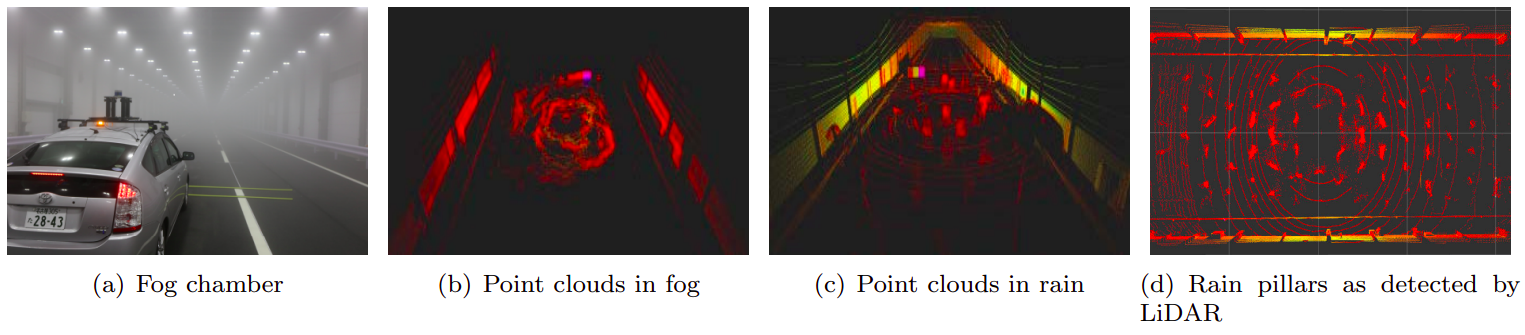
\includegraphics[width=0.9\textwidth]{images/lidar_issues.png}
    %                 \caption{LiDAR performance test \cite{Zhang2021Dec}}
    %                 \label{fig:lidar}
    %         \end{figure}

    %         \begin{figure}[h]
    %             \centering
    %             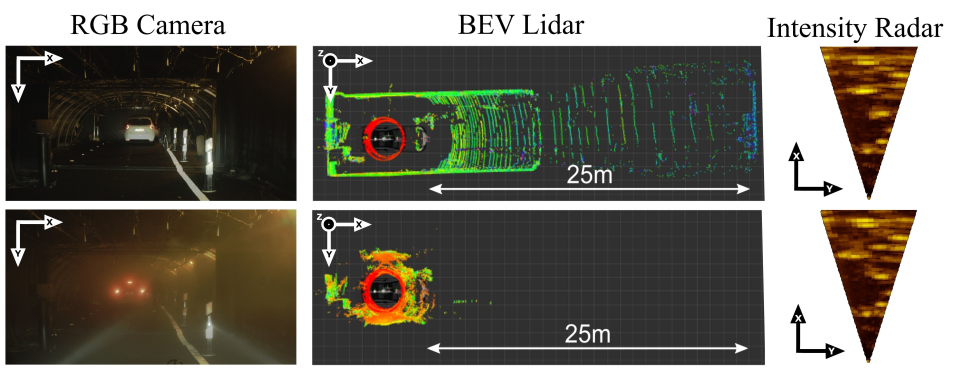
\includegraphics[width=0.8\textwidth]{images/lidar_in_fog.png}
    %             \caption{\centering 1st row: clear weather condition, 2nd row: with fog. Shows that lidar affects by the fog but radar intensity remains the same \cite{bijelic2020seeing}}
    %             \label{fig:lidar_in_fog}
    %         \end{figure}
        
    %     \item Radar is the third most crucial sensor in autonomous driving systems and is widely used in mass-produced cars for active safety functions, such as automatic emergency braking (AEB) and forward collision warning (FCW). However, its significance in perception tasks for autonomous driving is often underestimated. Unlike RGB cameras that utilize visible light bands (384--769 THz) and LiDARs that operate within infrared bands (361--331 THz), radar uses relatively longer wavelength radio bands (77--81 GHz), which ensures robust measurements in adverse weather conditions \cite{Paek2022Jun}. Ijaz et al. \cite{ijaz2012analysis} and Ismail \cite{gultepe2008measurements} report that radar exhibits lower attenuation in rainy conditions compared to LiDAR. At 77 GHz, radar's attenuation is approximately 3.5 times lower (10 dB/km) than that of LiDAR at 905 nm (35 dB/km), demonstrating superior robustness. Multiple experiments \cite{adams2012robotic, brooker2007seeing, xu2022learned, gourova2017analysis, zang2019impact} have shown that attenuation and backscattering for radar are negligible under dust, fog, snow, and light rain, while its performance degrades only in heavy rainfall. Figure \ref{fig:adverse_weather_influence_on_sensor} presents an example from the DENSE \cite{bijelic2020seeing} dataset where, under dense fog conditions, camera and LiDAR sensors fail to detect objects, yet radar can still identify the vehicle without any issues. A significant drawback of radar, however, is its low resolution, making it challenging to use for perception tasks. The radar point cloud is sparser than that of LiDAR, limiting its utility. Recently, the advent of next-generation 4D radar has shown promise in providing denser point clouds compared to conventional radar sensors. However, no publicly available dataset currently includes 4D radar data in adverse weather conditions.
        
    %     % four images
    %     \begin{figure}[ht]
    %         \centering
            
    %         \begin{subfigure}{.5\textwidth}
    %           \centering
    %           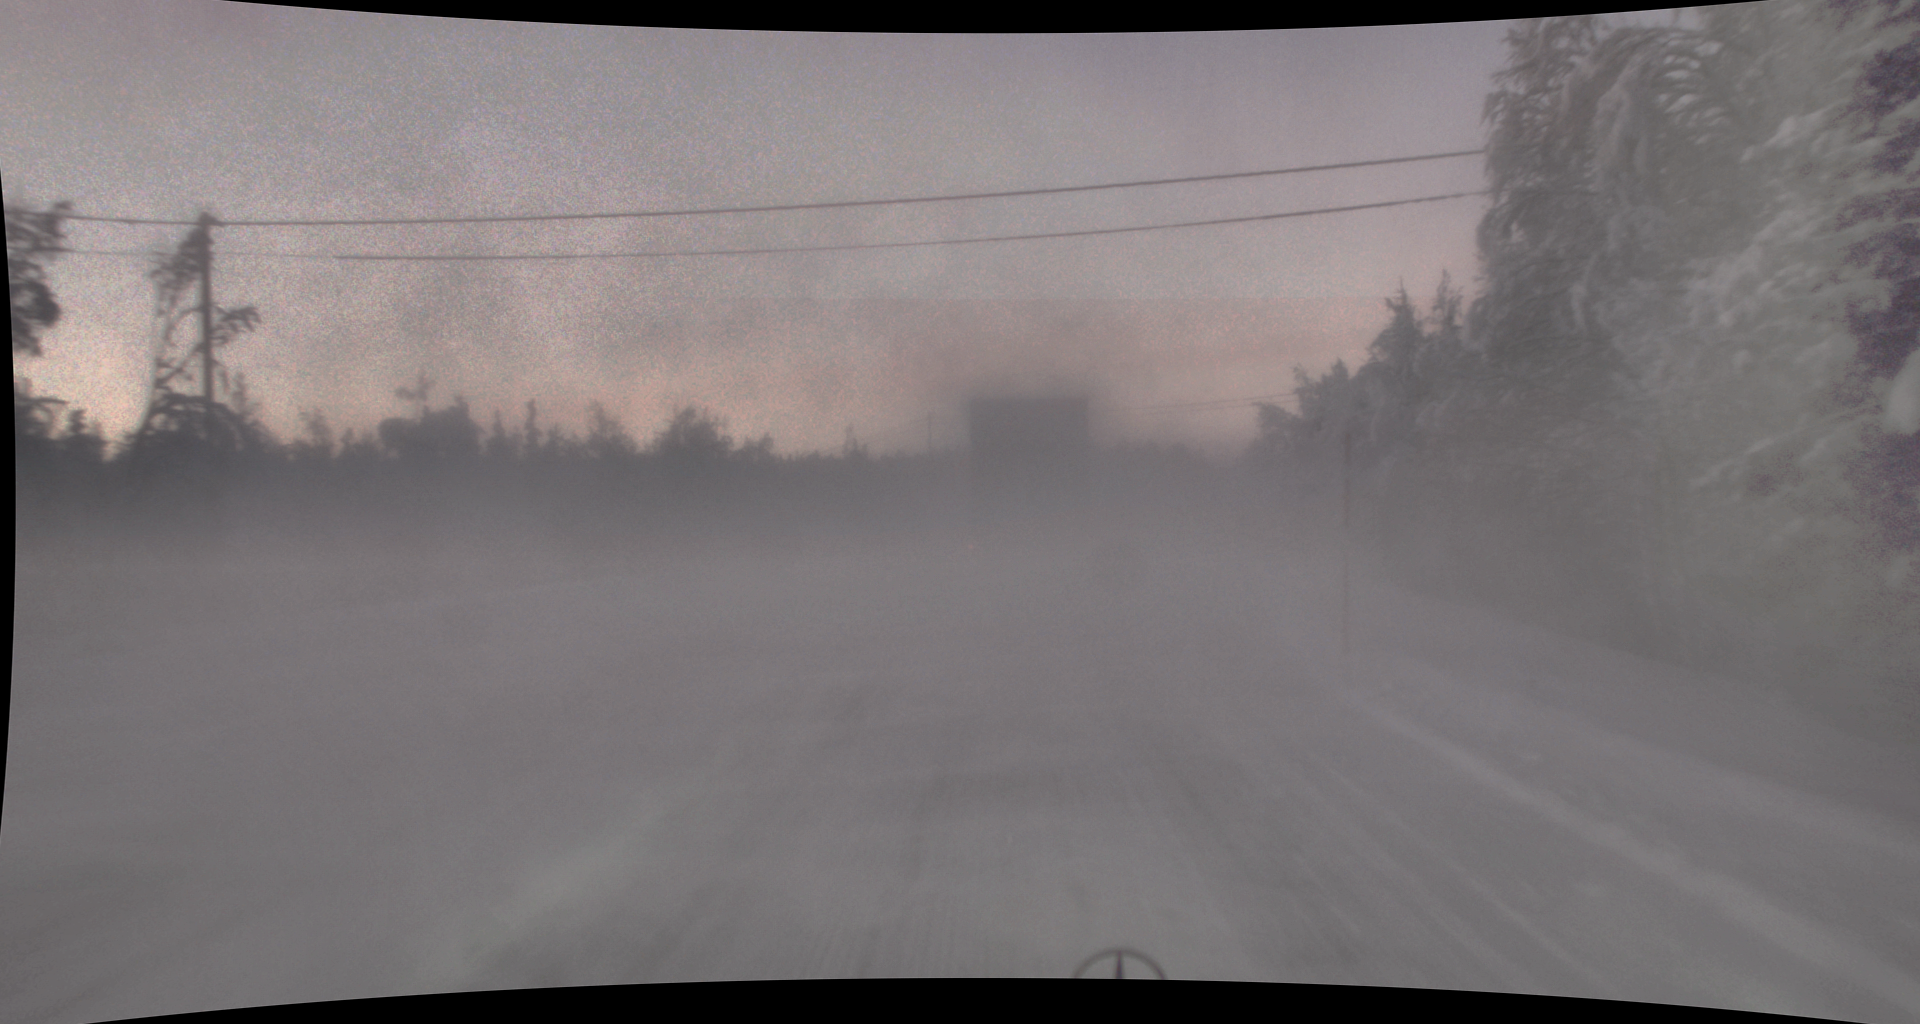
\includegraphics[width=.9\linewidth]{images/adverse_weather_influence_on_sensor/camera_1.png}
    %           \caption{Camera}
    %           \label{fig:sub1}
    %         \end{subfigure}%
    %         \begin{subfigure}{.5\textwidth}
    %           \centering
    %           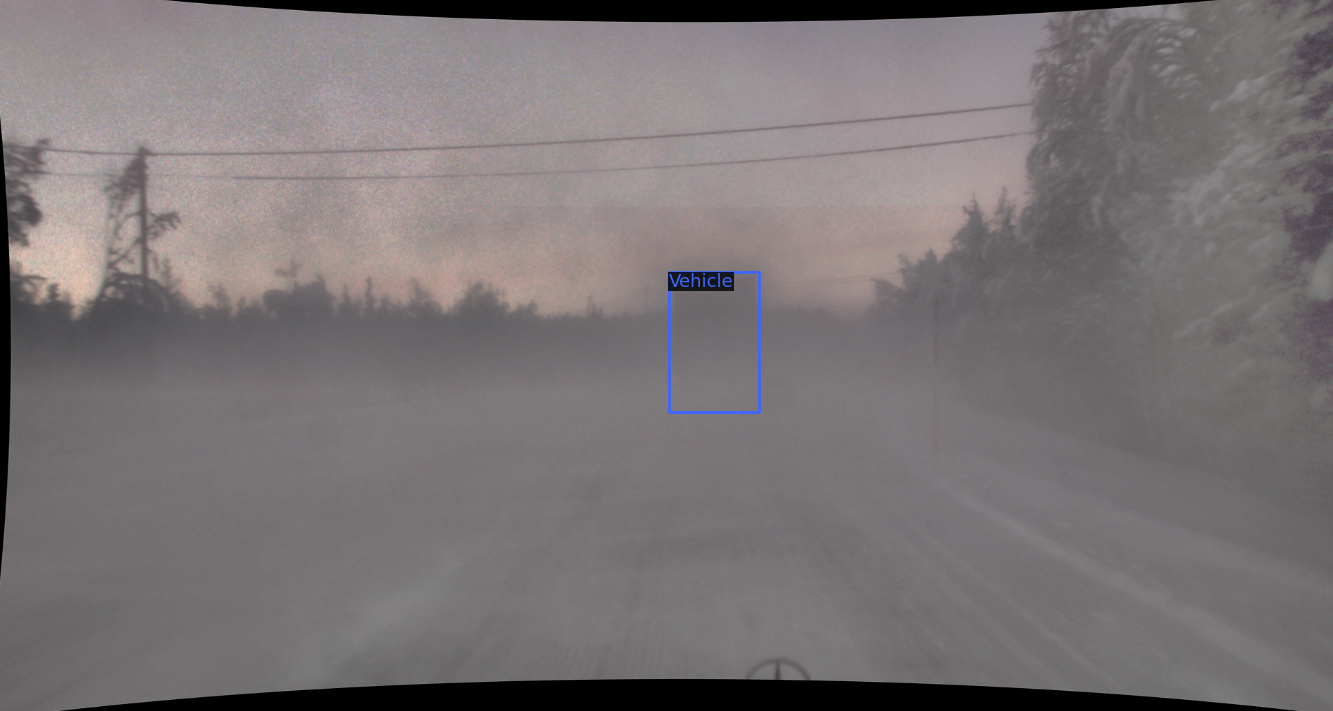
\includegraphics[width=.9\linewidth]{images/adverse_weather_influence_on_sensor/gt.png}
    %           \caption{Ground Truth}
    %           \label{fig:sub2}
    %         \end{subfigure}
            
    %         \begin{subfigure}{.5\textwidth}
    %           \centering
    %           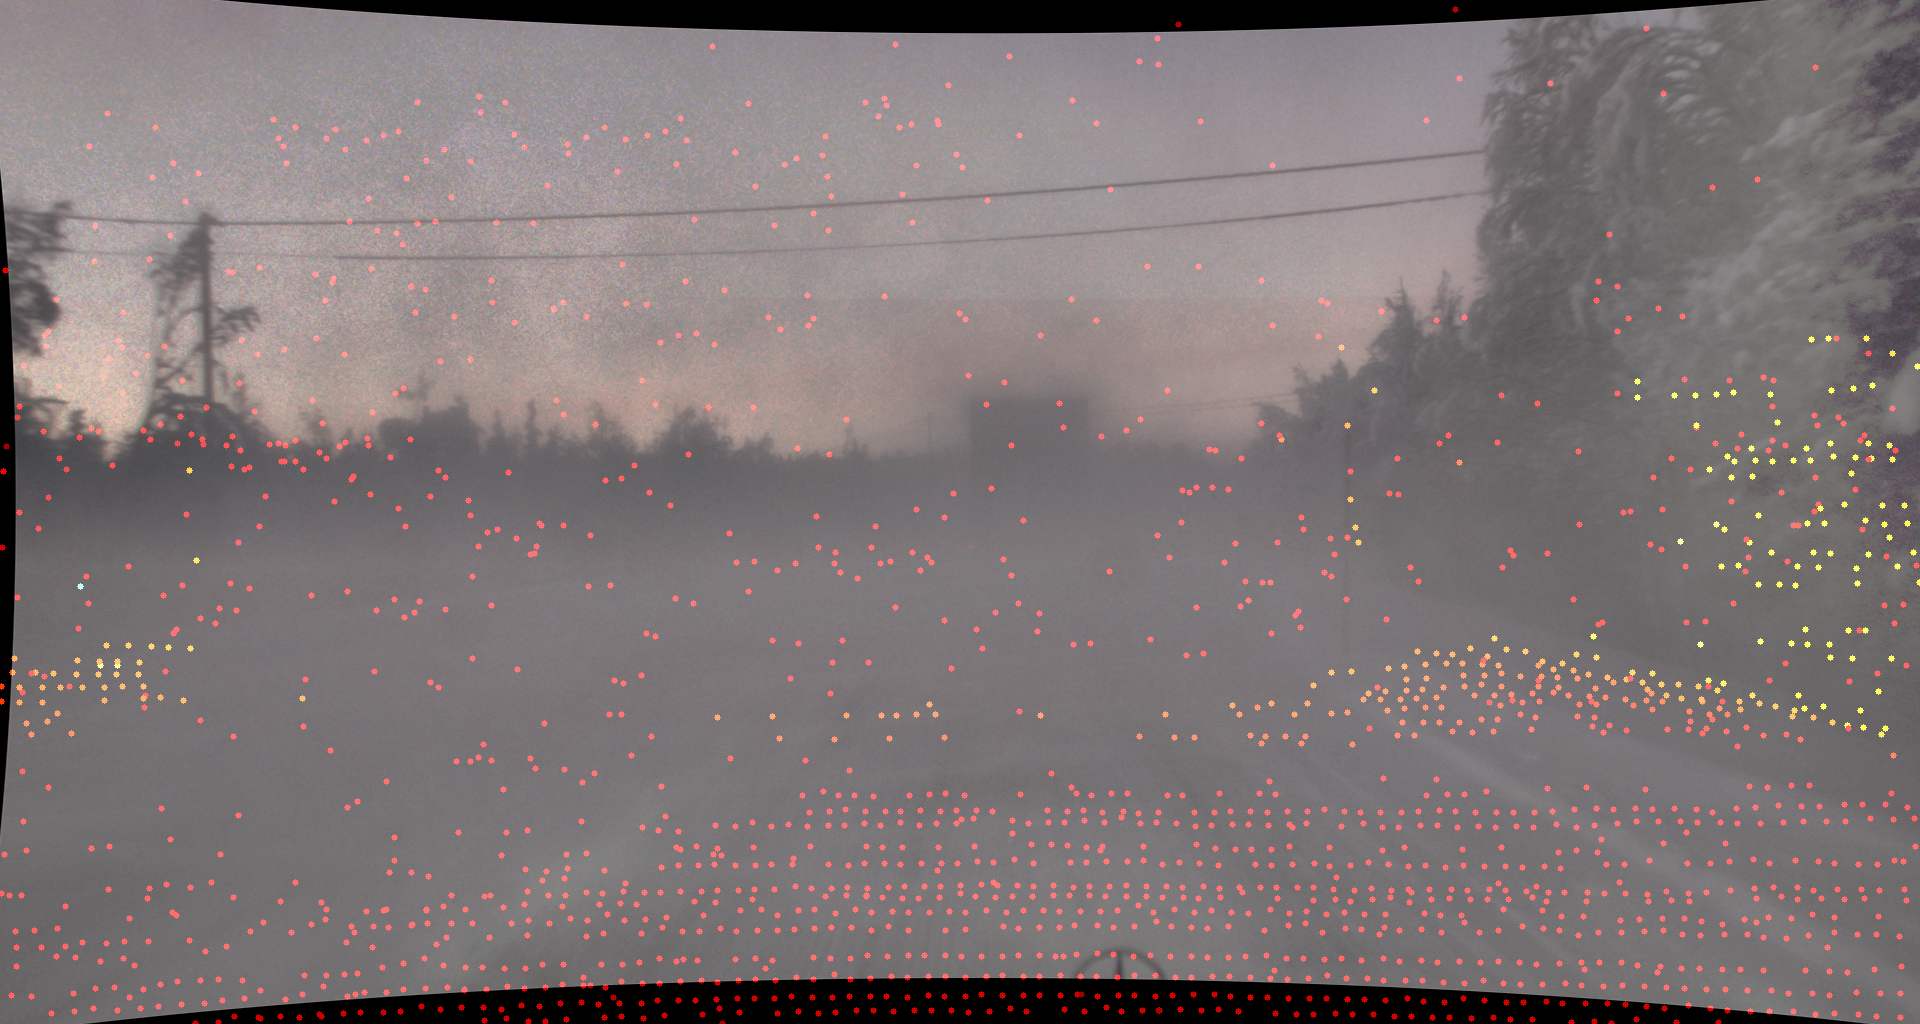
\includegraphics[width=.9\linewidth]{images/adverse_weather_influence_on_sensor/lidar_1.png}
    %           \caption{Lidar}
    %           \label{fig:sub3}
    %         \end{subfigure}%
    %         \begin{subfigure}{.5\textwidth}
    %           \centering
    %           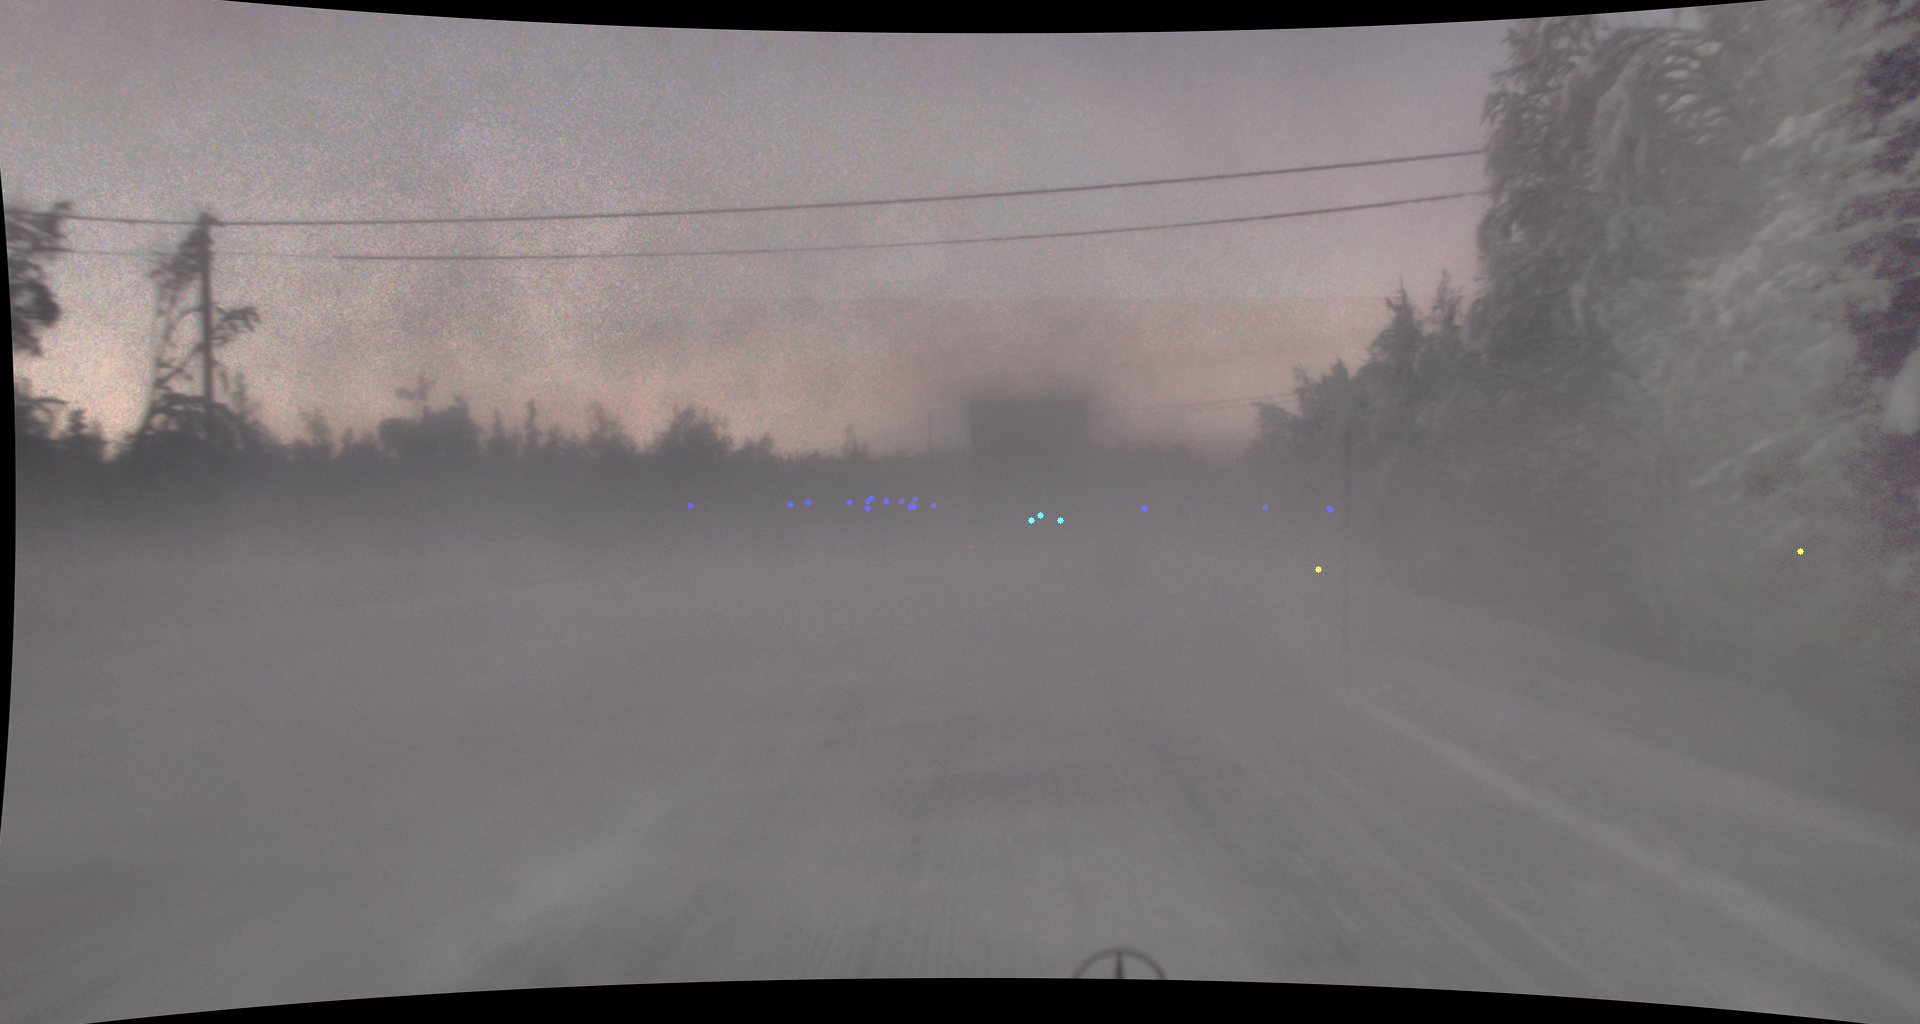
\includegraphics[width=.9\linewidth]{images/adverse_weather_influence_on_sensor/radar_1.png}
    %           \caption{Radar}
    %           \label{fig:sub4}
    %         \end{subfigure}
            
    %         \caption{\centering Dense fog influence on sensors (a sample from DENSE dataset \cite{bijelic2020seeing}) }
    %         \label{fig:adverse_weather_influence_on_sensor}
    %     \end{figure}


    %     % ===> Why do we need multimodal perception?
    %     \item By now, it’s almost well established that the LiDAR or Camera architecture alone is not going to navigate through adverse weather conditions with enough safety assurance. But two forces combining together would be a different story with the additional strength. The same can be seen as discussed before from the Figure \ref{fig:sensors_intro_1} and \ref{fig:sensors_intro_2}. As a result, groups from all over the world come up with their own permutation and combination with camera, LiDAR, radar, infrared camera, gated camera, stereo camera, weather stations and other weather-related sensors.
        
        
        
    % \end{itemize}

    In the evolving landscape of autonomous robotics, particularly in the domains of self-driving vehicles and autonomous drones, object detection stands as a paramount challenge in computer vision. These cutting-edge applications necessitate precise 2D or 3D bounding boxes for objects within complex and often unpredictable real-world environments. These scenarios commonly involve cluttered scenes, varying lighting conditions, and notably, adverse weather conditions. To tackle these multifaceted challenges, state-of-the-art autonomous vehicle systems are increasingly reliant on a suite of redundant sensor modalities. Recent studies, such as those by Caesar et al. \cite{caesar2020nuscenes}, Sun et al. \cite{Sun_2020_CVPR}, and Ziegler et al. \cite{ziegler2014making}, highlight this trend. These sensor modalities extend beyond traditional cameras and LiDAR, encompassing radar and emerging technologies like far-infrared (FIR) and near-infrared (NIR) sensors, which are proving instrumental in enabling reliable object detection in adverse conditions \cite{bijelic2020seeing}.

    For standard perception systems in autonomous vehicles, the camera remains an indispensable, yet highly vulnerable sensor to adverse weather conditions. Despite its high resolution, a camera's functionality can be severely compromised by a single water drop on the lens or emitter during rain \cite{mardirosian2021LiDAR}, as illustrated in Figure \ref{fig:camera_in_rain}. In conditions like heavy snow or hail, image intensity can fluctuate, and object edges may become obscured, leading to detection failures \cite{zang2019impact}. Additionally, cameras are susceptible to strong light interference, either from direct sunlight or artificial sources like urban light pollution, causing significant operational challenges \cite{acarballo2020libre}.

    \begin{figure}[h]
        \centering
        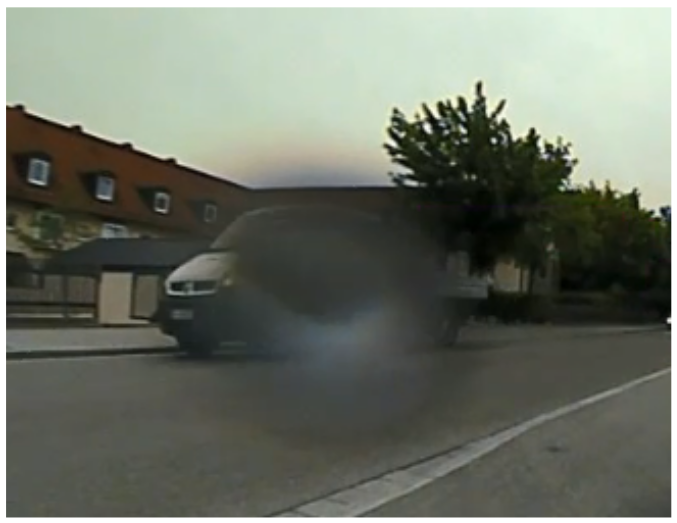
\includegraphics[width=0.5\textwidth]{images/rain_droplet.png}
        \caption{Van occluded by a water droplet on the lens \cite{Nobis2020May}}
        \label{fig:camera_in_rain}
    \end{figure}
    
    LiDAR, the second-most common sensor in autonomous driving systems, exhibits a different response to adverse weather. As Fersch et al. \cite{fersch2016influence} suggest, LiDAR sensors with small apertures are relatively unaffected by moderate rainfall. However, intense and uneven precipitation can generate fog clusters, potentially resulting in false obstacle detection by LiDAR systems. Hasirlioglu et al. \cite{hasirlioglu2016modeling} demonstrated that rainfall rates exceeding 40 mm/hr significantly reduce signal reflection intensity. Dense fog and smoke, along with strong light, can adversely affect LiDAR sensors in challenging conditions \cite{Zhang2021Dec, acarballo2020libre}. This is exemplified in Figure \ref{fig:lidar}, which showcases an instance of LiDAR's performance in fog, where it erroneously creates small false obstacle clouds. Similarly, Figure \ref{fig:lidar_in_fog} illustrates how LiDAR's ability to measure distances is compromised in foggy environments. This contrasts with radar technology, whose outputs remain largely unaffected under similar conditions. Such discrepancies highlight the limitations of LiDAR in adverse weather and the need for integrating complementary sensor modalities for enhanced reliability in autonomous driving systems.

    \begin{figure}[h]
        \centering
        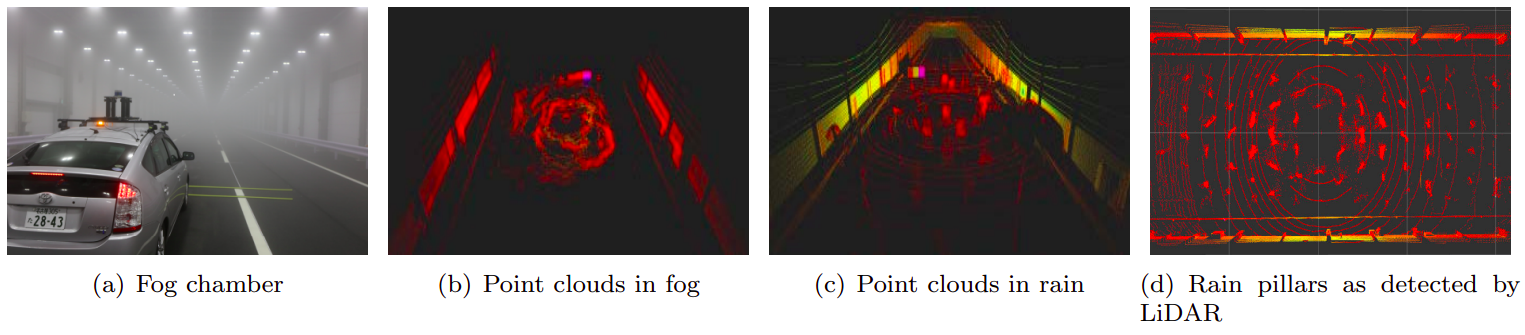
\includegraphics[width=0.9\textwidth]{images/lidar_issues.png}
        \caption{LiDAR performance test \cite{Zhang2021Dec}}
        \label{fig:lidar}
    \end{figure}

    \begin{figure}[h]
        \centering
        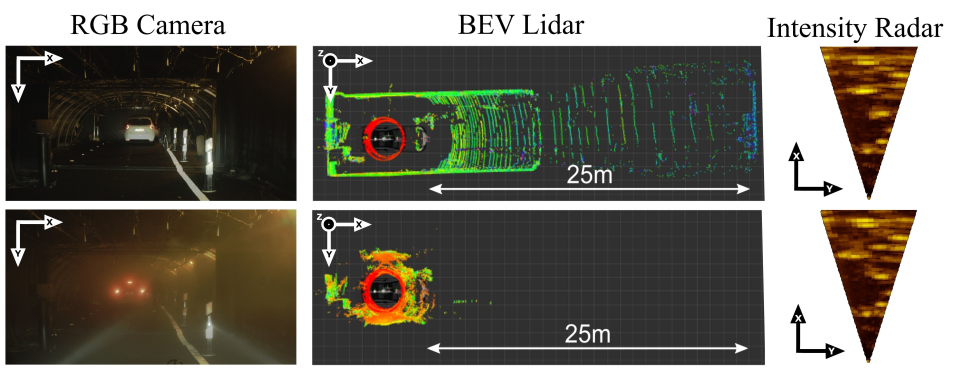
\includegraphics[width=0.8\textwidth]{images/lidar_in_fog.png}
        \caption{\centering 1st row: clear weather condition, 2nd row: with fog. Shows that lidar affects by the fog but radar intensity remains the same \cite{bijelic2020seeing}}
        \label{fig:lidar_in_fog}
    \end{figure}
    
    Radar, the third critical sensor in autonomous driving systems, is frequently used in mass-produced cars for active safety functions like Automatic Emergency Braking (AEB) and Forward Collision Warning (FCW). Its role in perception tasks for autonomous driving, however, is often undervalued. Unlike cameras operating in the visible light bands (384–769 THz) and LiDARs in the infrared bands (361–331 THz), radar utilizes longer wavelength radio bands (77–81 GHz). This attribute ensures its robust performance in adverse weather conditions \cite{Paek2022Jun}. Studies by Ijaz et al. \cite{ijaz2012analysis} and Ismail \cite{gultepe2008measurements} indicate radar's lower attenuation in rainy conditions compared to LiDAR. At 77 GHz, radar exhibits approximately 3.5 times less attenuation (10 dB/km) than LiDAR at 905 nm (35 dB/km), showcasing its superior robustness. Various experiments \cite{adams2012robotic, brooker2007seeing, xu2022learned, gourova2017analysis, zang2019impact} have demonstrated that radar's performance is minimally affected by dust, fog, snow, and light rain, although it degrades in heavy rainfall conditions. Figure \ref{fig:adverse_weather_influence_on_sensor} from the DENSE \cite{bijelic2020seeing} dataset exemplifies this, showing radar's ability to detect vehicles under dense fog conditions, where cameras and LiDAR fail. Nevertheless, radar's low resolution and sparser point clouds compared to LiDAR limit its utility in perception tasks. The emerging 4D radar technology, while promising denser point clouds, lacks public datasets in adverse weather conditions for validation.

    % four images
    \begin{figure}[ht]
        \centering
        
        \begin{subfigure}{.5\textwidth}
            \centering
            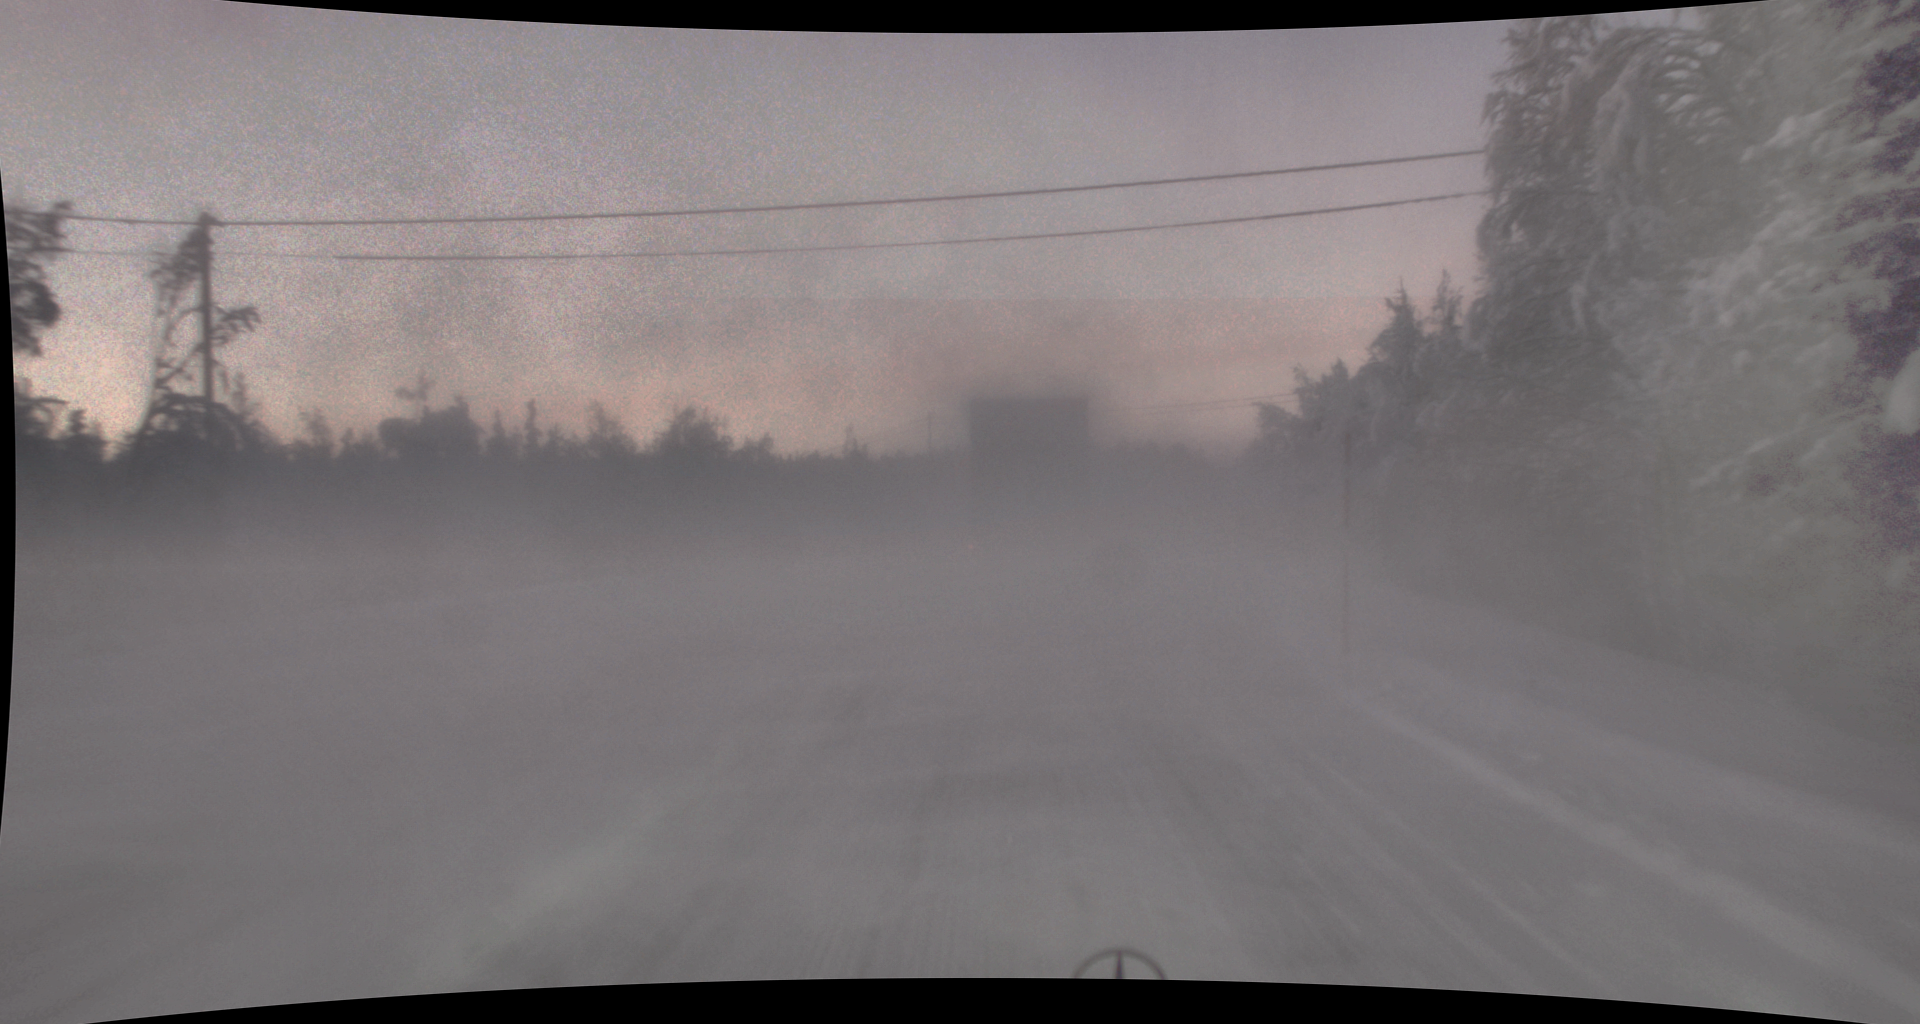
\includegraphics[width=.9\linewidth]{images/adverse_weather_influence_on_sensor/camera_1.png}
            \caption{Camera}
            \label{fig:sub1}
        \end{subfigure}%
        \begin{subfigure}{.5\textwidth}
            \centering
            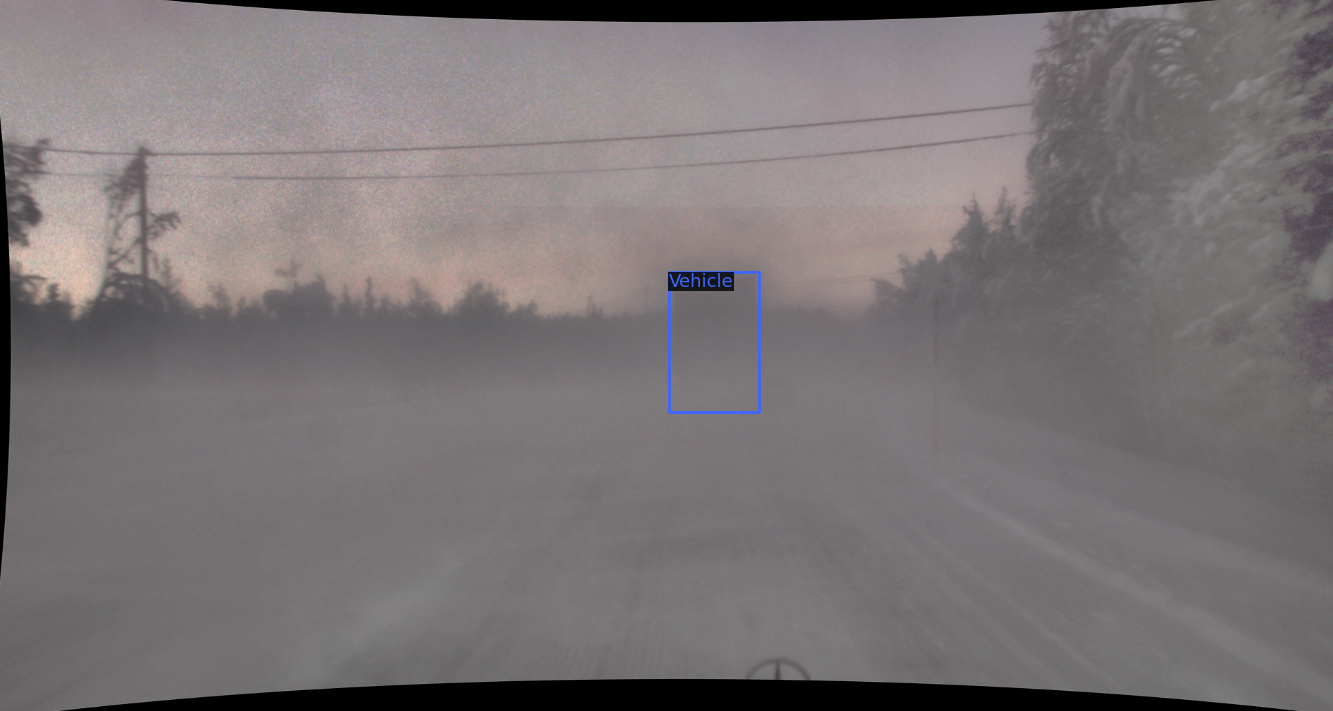
\includegraphics[width=.9\linewidth]{images/adverse_weather_influence_on_sensor/gt.png}
            \caption{Ground Truth}
            \label{fig:sub2}
        \end{subfigure}
        
        \begin{subfigure}{.5\textwidth}
            \centering
            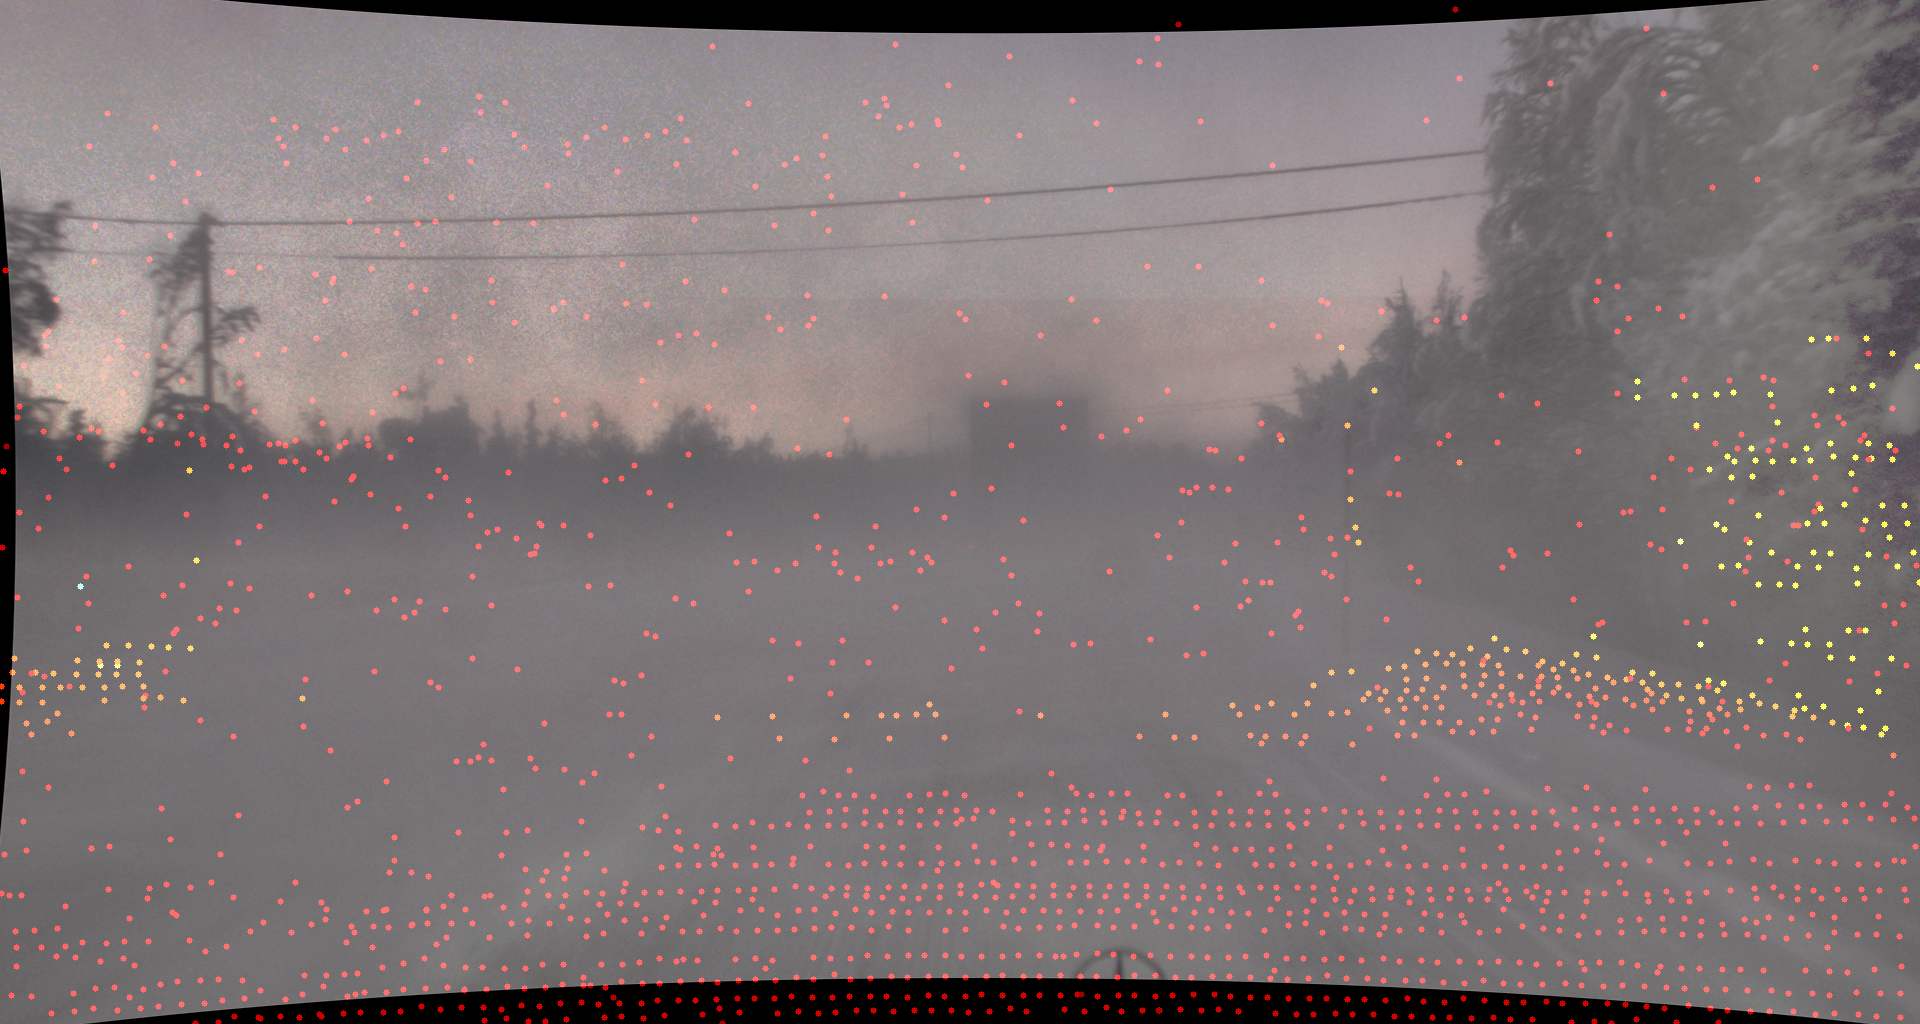
\includegraphics[width=.9\linewidth]{images/adverse_weather_influence_on_sensor/lidar_1.png}
            \caption{Lidar}
            \label{fig:sub3}
        \end{subfigure}%
        \begin{subfigure}{.5\textwidth}
            \centering
            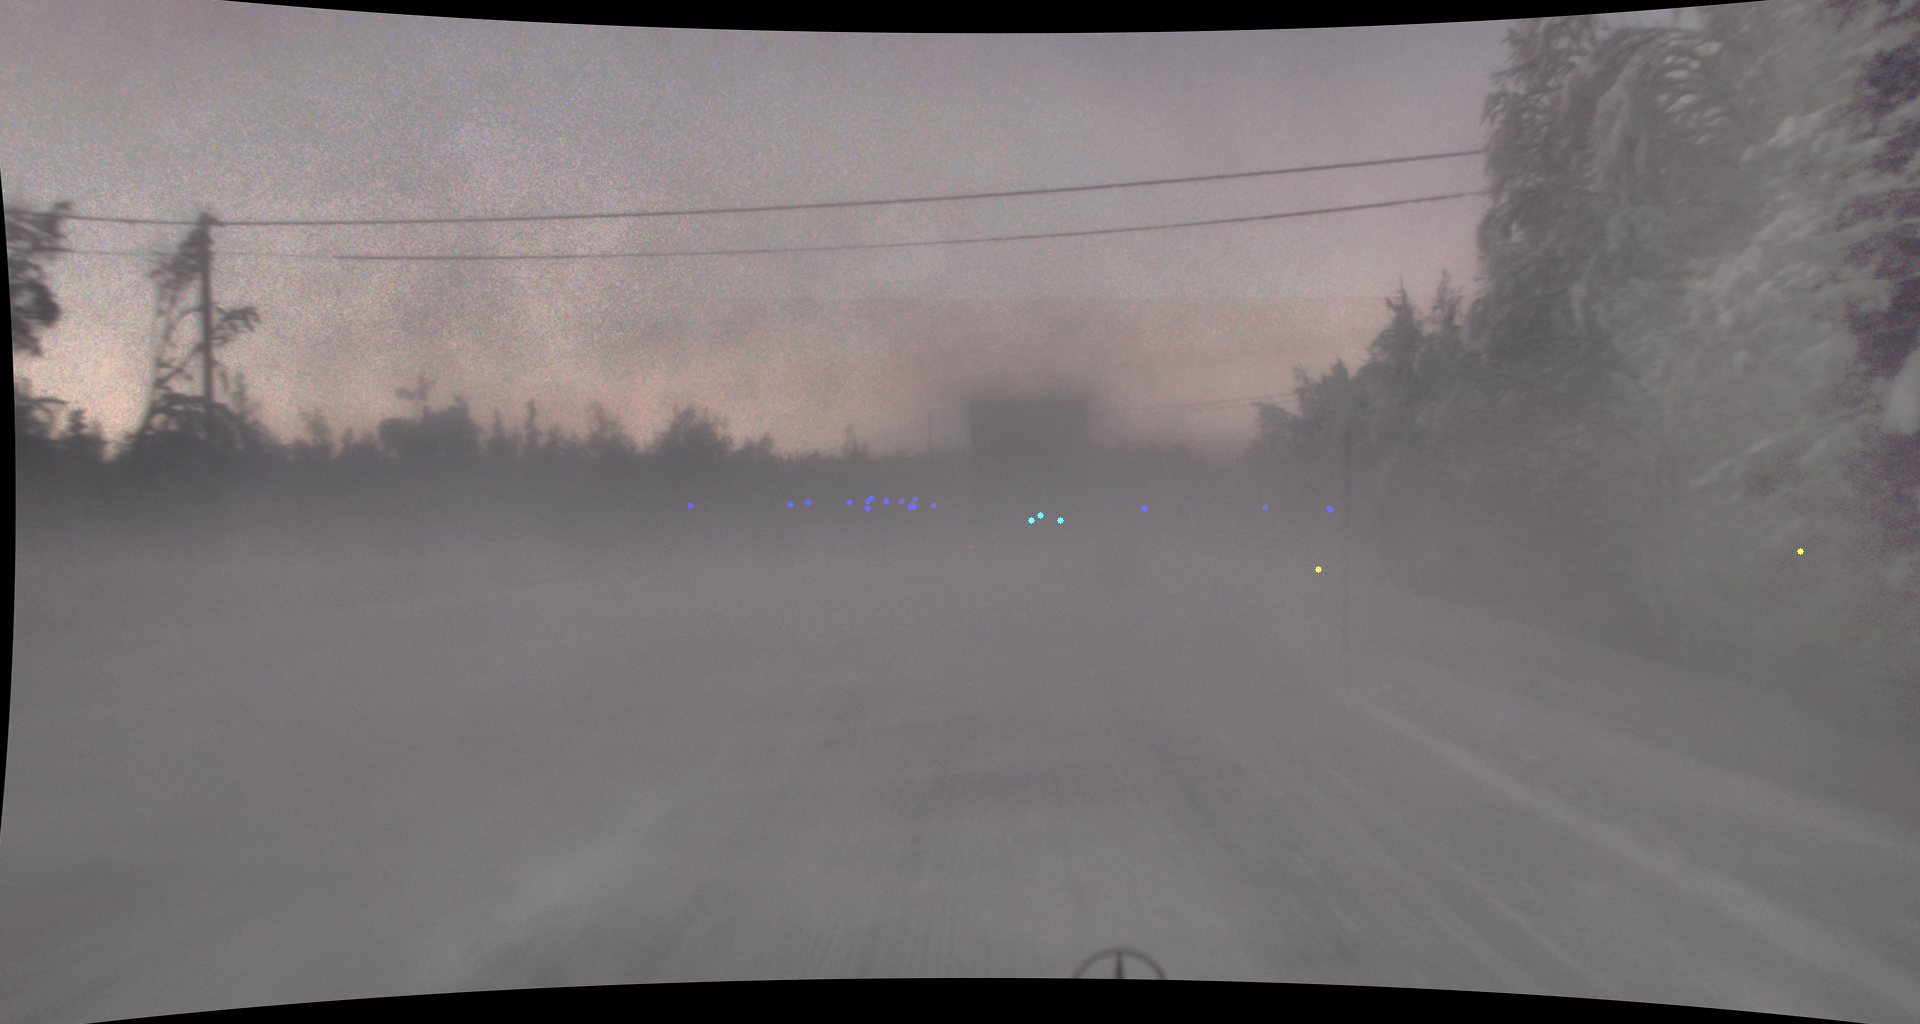
\includegraphics[width=.9\linewidth]{images/adverse_weather_influence_on_sensor/radar_1.png}
            \caption{Radar}
            \label{fig:sub4}
        \end{subfigure}
        
        \caption{\centering Dense fog influence on sensors (a sample from DENSE dataset \cite{bijelic2020seeing}) }
        \label{fig:adverse_weather_influence_on_sensor}
    \end{figure}
    
    The combination of LiDAR and camera technologies alone has proven insufficient for navigating through adverse weather conditions with adequate safety assurance. However, the integration of these with radar, infrared cameras, gated cameras, stereo cameras, weather stations, and other weather-related sensors presents a new paradigm in autonomous vehicle perception. This multimodal sensor fusion, as evidenced in Figures \ref{fig:sensors_intro_1} and \ref{fig:sensors_intro_2}, offers a composite strength that individual systems lack. Consequently, research groups worldwide are exploring various permutations and combinations of these sensors to enhance the reliability and safety of autonomous driving systems in challenging weather conditions.



    \section{Multimodal Sensor Fusion}

    % \begin{itemize}
        
    %     \item Radecki et al. \cite{radecki2016all} conducted a comprehensive review, investigating the efficacy of various sensors in a range of weather conditions including wet conditions, day and night, cloudy skies, glare, and dust. They engineered a robust system capable of tracking and classifying objects through a real-time, joint probabilistic perception algorithm. This advanced algorithm employs a dynamic selection of sensor subsets that are particularly suited to the prevailing weather conditions. The system not only elevates the general lower bound of perception ability but also optimizes its robustness and reliability through intelligent weighting of sensors and precise quantification of parameters based on the specific weather context. Such a design emphasizes the crucial role of real-time strategy shifts and intelligent sensor subset selection in maximizing the accuracy and reliability of multimodal perception systems.
    %     % 2016
    %     \item Limitations of Radecki et al.'s \cite{radecki2016all} study include an emphasis on optimal weather conditions and a lack of investigation into heavy traffic or urban areas, as well as deep learning-based fusion techniques. Future research should consider these limitations and explore the use of proposed Similarly-based methods for object detection in adverse weather datasets.
        
    %     \item FLIR System Inc. \cite{fused_aeb} and VSI Labs \cite{VSILabs} conducted a test on the first ever fused automated emergency braking (AEB) sensor suite in 2019, consisting of a thermal long-wave infrared (LWIR) camera, a radar, and a visible camera. The LWIR camera captures wavelengths ranging from 8 µm to 14 µm and operates under ambient temperature, known as the uncooled thermal camera. The sensor suite was evaluated alongside several cars equipped with AEB systems employing radar and visible cameras under various conditions including day-time, nighttime, and tunnel exit into sun glare. The comparison results indicate that while most AEB systems perform adequately during the day, the standard AEB almost collided with every mannequin under adverse conditions, whereas the LWIR sensor suite avoided any collision. This study underscores the potential of fusing camera and radar in challenging weather situations.
    %     % 2019
    %     \item The work done by FLIR System Inc. \cite{fused_aeb} and the VSI Labs \cite{VSILabs} by using a thermal camera for fusion as one of the sensors, which raises the concerns of the durability of such temperature-sensitive devices in real environments. This needs further validation in real environments in the future to ensure their usefulness in adverse weather conditions \cite{zang2019impact}.
        
    %     \item To address the problem of when to fuse the data in the neural network architecture, Nobis et al. \cite{nobis2019deep} proposed a CameraRadarFusionNet (CRF-Net), which was inspired from camera-LiDAR fusion \cite{yu2019multi} and \cite{caltagirone2019lidar}, to learn at which level the fusion of the sensor data was the most beneficial for the detection task. They used nuScenes \cite{caesar2020nuscenes} dataset and released their own TUM dataset. Furthermore, they introduced a new training strategy to focus the learning on a specific sensor type, which was called BlackIn. For feature fusion, the element-wise addition was adopted as the fusion operation. Their fusion method outperformed the image-only network on both datasets, which again shows the importance of fusing radar data into the detection task.
    %     % 2019
    %     \item Nobis et al. \cite{nobis2019deep} proposed the CameraRadarFusionNet (CRF-Net) to learn the optimal level for sensor data fusion in the neural network architecture for detection tasks. While their fusion method outperformed the image-only network on nuScenes \cite{caesar2020nuscenes} and their own TUM dataset, the improvement in detection performance was limited. The element-wise addition used for feature fusion was a simple method, and the baseline image network's performance was only slightly lower than the CRF-Net's performance. Additionally, the study did not provide an RGB sensor ablation study, so it was unclear whether their system was robust in the case of camera failure. According to Safa et al. \cite{safa2021fail}, the performance could be further improved by pre-processing the radar data before fusion.
        
    %     \item Yang et al. \cite{yang2020radarnet} proposed RadarNet for object detection and velocity estimation, that leverages radar and LiDAR sensors for perception. RadarNet employs early fusion to learn joint representations from both sensors and late fusion to incorporate the radial velocity evidence of radar and enhance the estimated object velocity. The authors evaluated their approach on the nuScenes dataset \cite{caesar2020nuscenes}.
    %     \item In the RadarNet architecture, proposed by Yang et al. \cite{yang2020radarnet}, the radar sensor data used from the nuScenes dataset, which has a very low resolution and hence it's not a good choice for studying the role of radar in perception. Object detection using radars is limited by low resolution and erroneous elevation estimates \cite{ulrich2021deepreflecs} \cite{drews2022deepfusion}. Therefore, one possible improvement is to include the radar sensor used in K-Radar dataset, which is a 4D radar with elevation angle of 30 degrees compare to 1 or 2 degrees for conventional radars, can be used to improve the performance of the RadarNet architecture.
        
    %     \item Bijelic et al. \cite{bijelic2020seeing} from Mercedes-Benz AG conducted a study on improving detection performance in adverse weather conditions using a deep multimodal sensor fusion approach. The authors equipped their test vehicle with various sensors, including stereo RGB cameras, a NIR camera, a 77 GHz radar, two LiDARs, an FIR camera, a weather station, and a road-friction sensor. They proposed an entropy-steered fusion approach where regions with low entropy were attenuated while entropy-rich regions were amplified during feature extraction. The exteroceptive sensor data were concatenated and trained using clear weather data, demonstrating strong adaptation to unseen adverse weather data. The fusion network was designed to generalize across different scenarios, and all the sensor data were projected into the camera coordinate system to ensure consistency. The fused detection performance outperformed LiDAR or image-only approaches under fog conditions.
    %         % \item TODO: add images
    %         \begin{figure}[h]
    %             \centering
    %             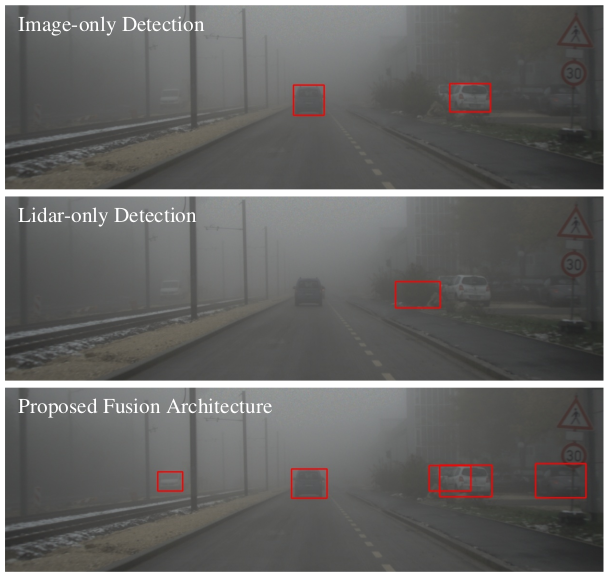
\includegraphics[width=0.4\textwidth]{images/seeing_through_fog.png}
    %             \caption{Highlighting the significance of fusing multimodal sensor data \cite{bijelic2020seeing}}
    %             \label{fig:seeing_through_fog}
    %         \end{figure}
    %     \item Bijelic et al. \cite{bijelic2020seeing} also provided the SeeingThroughFog or DENSE dataset for further research on multimodal sensor fusion in adverse weather conditions. This dataset comprises 10,000 km of driving data in Northern Europe, recorded during February and December 2019, under varying weather and illumination conditions. The dataset includes annotations for 5.5 k clear weather frames, 1 k dense fog frames, 1 k light fog frames, and 4 k frames captured in snow/rain.
    %     % 2020
    %     \item The study conducted by Bijelic et al. \cite{bijelic2020seeing} presents a multimodal sensor fusion approach that outperforms LiDAR or image-only approaches under fog conditions. However, one issue is that some essential radar information may be lost during the projection transformation used by the proposed method, leading to a loss of spatial information. Additionally, the large number of sensors required by the approach exceeds the typical expectations for an autonomous driving system, making it challenging to implement in real-world scenarios. The response and reaction time of the algorithm may also become a concern due to the bulk amount of data from multiple sensors. While the study demonstrated strong adaptation to adverse weather data, the performance of the radar used was limited by its low azimuth and elevation resolution \cite{Zhang2021Dec}. To address these limitations, future work could focus on improving the network architecture by using a higher resolution radar and using a transformer-based approaches to improve the performance of the sensor fusion approach in adverse weather conditions.
        
    %     % 2021
    %     \item Liu et al. \cite{liu2021robust} presented a novel approach to enhance the target recognition and tracking by fusing radar and camera data. In this approach, radar is considered as the primary sensor, and camera data is used as secondary information to complement the radar measurements. The authors evaluated the performance of their approach in challenging weather conditions, including rain and fog, as well as low visibility scenarios during nighttime. The experimental results revealed that radar-based detection exhibited high accuracy in detecting moving targets in wet weather, while the camera was more effective in target classification. Furthermore, the fusion of radar and camera data showed superior performance compared to LiDAR-based detection methods by over 33\%.
        
    %     % 2021
    %     \item Qian et al. \cite{qian2021robust} introduced a Multimodal Vehicle Detection Network (MVDNet) featuring LiDAR and radar. In the network architecture, MVDNet has a two-stage attention block in the fusion module. It first applied self-attention to each modality to extract features and then mixed them with region-wise features through cross attentions. Experiments showed that the fusion mechanism performs robustly in foggy weather. The authors trained and evaluated the model performance on DENSE \cite{bijelic2020seeing} and the Oxford Radar Robotcar \cite{barnes2020oxford} datasets. And the evaluation shows much better performance than LiDAR alone in fog conditions.
    %     % 2021
    %     \item Qian et al. \cite{qian2021robust} proposed a Multimodal Vehicle Detection Network (MVDNet) that combines LiDAR and radar data using a two-stage attention block in the fusion module. Despite demonstrating robust performance in foggy weather conditions, the study has some limitations. Firstly, the misalignment between the LiDAR and radar data in the dataset is not corrected, which can affect the MVDNet's performance. Secondly, the simple label assignment strategy used in the loss computation procedure and the region-of-interest (ROI) assisted fusion design limits the model's performance. These factors suggest that there is room for improvement in the model's design, which could potentially be addressed by more advanced fusion techniques and better label assignment strategies \cite{yang2022ralibev}.
        
    %     \item Rawashdeh et al. \cite{rawashdeh2021drivable} developed a CNN-based sensor fusion approach for detecting drivable paths using cameras, LiDAR, and radar, which was evaluated using the DENSE dataset \cite{bijelic2020seeing}. Their multi-stream encoder-decoder network was designed to compensate for the asymmetric degradation of the input sensors at the highest level. The depth and number of blocks for each sensor in the architecture were determined by their respective input data densities, with the camera having the highest density, followed by LiDAR, and radar having the lowest. The fully connected network's outputs were reshaped into a 2-D array that was input to the decoder. The researchers showed that their model could effectively disregard road lines and edges that might otherwise cause false interpretations and accurately delineate the general drivable area.
    %     \item Rawashdeh et al. \cite{rawashdeh2021drivable} proposed a multimodal fusion approach for drivable path detection in poor weather conditions. However, the proposed method lacks a comparison with other state-of-the-art methods and does not investigate the real-time processing requirements and computational cost of the proposed algorithm, which could limit its practical applicability \cite{rawashdeh2021drivable}.
        
    %     % My chosen method 1, SAF-FCOS
    %     \item The paper by Chang et al. \cite{chang2020spatial} introduces a novel method for enhancing obstacle detection in autonomous driving systems. This method, called spatial attention fusion (SAF), effectively integrates data from millimeter-wave (mmWave) radar and camera sensors. SAF addresses the sparsity of radar points by generating an attention weight matrix that distinctively fuses vision features, diverging from traditional concatenation or element-wise addition fusion methods. This method can be integrated into the feature-extraction stage of existing deep learning object detection frameworks, facilitating end-to-end training. Additionally, the paper presents a generation model that converts radar points into images for neural network training. This type of image projection called radar imagery. The paper's findings indicate that this fusion approach significantly improves performance on nuScenes \cite{caesar2020nuscenes} dataset.
        
    %     % My chosen method 2, HRFuser
    %     \item Another work by Broedermann et al. \cite{broedermann2022hrfuser} presents an extended work on HRNet \cite{wang2020deep} and HRFormer \cite{yuan2021hrformer} to integrate multimodal sensors into a single network. It introduces HRFuser, a versatile, multi-resolution, multi-sensor fusion architecture that can efficiently integrate an arbitrary number of sensors like lidar, radar, and gated cameras, alongside standard cameras. HRFuser is built on the HRNet and HRFormer paradigms, preserving high-resolution representations and incorporating a novel multi-window cross-attention (MWCA) block for effective fusion across multiple resolutions. The system's generic design allows for easy scalability with various sensors without the need for specialized components for each sensor. Extensive testing on major autonomous driving datasets, including nuScenes \cite{caesar2020nuscenes}, and DENSE \cite{bijelic2020seeing}, demonstrates HRFuser's superior performance over existing camera-only networks and sensor fusion methods, proving its efficacy in both standard and adverse weather conditions. HRFuser's adaptability to different sensor sets and its ability to selectively focus on relevant features from high-resolution data of additional sensors mark a significant advancement in the field of 2D object detection.
        
    %     % My chosen method 3, MT-DETR
    %     \item Recent work by Chu et al. \cite{chu2023mt} proposes a novel end-to-end multimodal multistage object detection network called MT-DETR (MulTi-sensor MulTimodal DTtection TRansformer) that leverages data from multiple sensors - camera, lidar, radar and time - to achieve robust detection, especially in adverse weather conditions. Here time modality is an additional binary image input to inform model about day or night. It employs specialized fusion modules - Residual Fusion Module (RFM) and Confidence Fusion Module (CFM) for hierarchical cross-modal feature fusion. The network also uses a Residual Enhancement Module (REM) to strengthen individual sensor branches. A multi-stage loss function further regularizes feature learning across modalities. Extensive experiments on the publicly available DENSE \cite{bijelic2020seeing} dataset demonstrate that MT-DETR significantly outperforms existing unimodal and multimodal detection methods. Notably, when additionally trained on realistic synthetic foggy data generated by a novel camera-lidar synthesis algorithm, the performance boost is even higher.
        
    %     TODO: write about my choosen methods limitations
        
    %     \item Since most of the advance multimodal sensor fusion techniques, including state-of-the-art ones, are developed on clear weather datasets without paying special attention to the adverse weather conditions. And many of them use LiDAR and camera \cite{feng2020deep} as the primary sensors. This could be because of the availability of the datasets. Hence, there is a need to study the performance of these advance deep learning techniques in adverse weather conditions with the combination of other sensors like radar, thermal camera, infrared camera, etc.
      
    %     \item Currently, there is no general guideline available for the design of network architecture in multimodal sensor fusion, and several questions remain unanswered. According to Feng et al. \cite{feng2020deep}, these include 
    %     \begin{itemize}
    %           \item "what to fuse," such as LiDAR, radar, color camera, thermal camera, event camera, or ultrasonic sensors; 
    %           \item "how to fuse," which can include addition or mean, concatenation, ensemble methods, or mixture of experts; 
    %           \item "when to fuse," which can involve early, mid, late, or a combination of all fusion methods.
    %     \end{itemize}
  
    %     \item The lack of comparison with alternative models or datasets is a limitation of previous studies on multimodal sensor fusion. Many studies have only shown results for their own baseline models and custom datasets, which limits the generalization of their findings.
        
    %     \item While recent multimodal datasets have released baseline models with simple fusion methods, the use of more advanced fusion methods, such as transformer-based or tightly-coupled fusion, has the potential to improve their performance.
  
    %     \item Temporal information is a crucial aspect of sensor fusion, but very few multimodal fusion algorithms have been developed to handle this type of data \cite{bijelic2020seeing}. Although this project does not consider the temporal information in the fusion process, it is still a promising area for future research.
  
    %     \item There is a dearth of work in the literature utilizing 4D imaging radar sensor especially for adverse weather conditions, which is a promising area for future research. \cite{Zhou2022May}

    % \end{itemize}


    The concept of multimodal sensor fusion has become increasingly pivotal in the field of object detection, particularly under adverse weather conditions. This approach integrates various sensor inputs to enhance perception and object detection capabilities, addressing the limitations inherent to individual sensors. A notable contribution in this field is the work of Radecki et al. \cite{radecki2016all}, who conducted a thorough review of sensor efficacy across diverse weather conditions, including wet environments, varying light conditions, and dusty atmospheres. They developed a sophisticated system capable of object tracking and classification through a real-time, joint probabilistic perception algorithm. This algorithm dynamically selects the most appropriate sensor subsets based on prevailing weather conditions. By intelligently weighting sensors and accurately quantifying parameters specific to each weather scenario, the system not only improves the baseline of perception ability but also enhances its robustness and reliability. This work underscores the importance of real-time strategy adaptation and smart sensor subset selection in maximizing the accuracy and dependability of multimodal perception systems.

    However, Radecki et al.'s study \cite{radecki2016all} has certain limitations, notably its focus on optimal weather conditions and the omission of heavy traffic and urban environments. Additionally, the study does not explore deep learning-based fusion techniques. Future research could address these gaps by employing similar approach for object detection in challenging weather datasets.

    In 2019, FLIR System Inc. \cite{fused_aeb} and VSI Labs \cite{VSILabs} tested the first-ever fused Automated Emergency Braking (AEB) sensor suite, comprising a thermal long-wave infrared (LWIR) camera, a radar, and a visible camera. The LWIR camera, operating in the 8 µm to 14 µm range at ambient temperature, was part of this groundbreaking sensor suite. The suite's performance was evaluated against standard AEB systems using radar and visible cameras under various conditions, including daytime, nighttime, and transitions from tunnel exits into sun glare. The results revealed that while most AEB systems function effectively during the day, they almost invariably failed under adverse conditions, often colliding with mannequins. In stark contrast, the LWIR sensor suite successfully avoided collisions in these challenging scenarios, highlighting the efficacy of fusing camera and radar data in adverse weather conditions.

    However, the use of a thermal camera as part of the sensor fusion raises concerns about the durability of such temperature-sensitive devices in real-world settings, necessitating further validation to ascertain their effectiveness in adverse weather \cite{zang2019impact}.

    Another significant development in multimodal sensor fusion is the CameraRadarFusionNet (CRF-Net) proposed by Nobis et al. \cite{nobis2019deep}. Inspired by previous works on camera-LiDAR fusion \cite{yu2019multi, caltagirone2019lidar}, the CRF-Net was designed to determine the most beneficial stage for sensor data fusion within a neural network architecture for detection tasks. Utilizing the nuScenes \cite{caesar2020nuscenes} dataset and their own TUM dataset, they introduced a novel training strategy, BlackIn, focusing on a specific sensor type. The fusion method employed, element-wise addition, demonstrated superior performance over an image-only network on both datasets, underscoring the significance of incorporating radar data into detection tasks.

    Nevertheless, Nobis et al.'s approach \cite{nobis2019deep} exhibited only marginal improvements in detection performance over the baseline image network. The absence of an RGB sensor ablation study in their work left questions about the system's robustness in case of camera failure. According to Safa et al. \cite{safa2021fail}, pre-processing the radar data before fusion could further enhance performance, suggesting an area for potential improvement in future research endeavors.

    Building on the concept of multimodal sensor fusion, Yang et al. \cite{yang2020radarnet} introduced RadarNet, a novel framework for object detection and velocity estimation. RadarNet is distinctive for its dual strategy of leveraging both radar and LiDAR sensors for perception. It employs an early fusion technique to learn joint representations from these sensors, while its late fusion phase incorporates radar's radial velocity evidence to enhance object velocity estimation. This approach was rigorously evaluated using the nuScenes dataset \cite{caesar2020nuscenes}. However, a limitation of RadarNet, as noted by Yang et al. \cite{yang2020radarnet}, lies in the radar sensor data from the nuScenes dataset, which is characterized by low resolution, thus restricting its effectiveness in object detection. This issue of low resolution and erroneous elevation estimates, as highlighted in studies like Ulrich et al. \cite{ulrich2021deepreflecs} and Drews et al. \cite{drews2022deepfusion}, suggests a potential improvement for RadarNet: the integration of a higher-resolution radar, such as the one from the K-Radar dataset. This 4D radar, with a significantly wider elevation angle, could enhance the performance of RadarNet, overcoming the limitations of conventional radars.

    In a similar vein, Bijelic et al. \cite{bijelic2020seeing} from Mercedes-Benz AG conducted an extensive study focusing on enhancing detection performance in adverse weather through deep multimodal sensor fusion. Their experimental setup included a diverse array of sensors on their test vehicle, including stereo RGB cameras, a NIR camera, a 77 GHz radar, dual LiDARs, an FIR camera, a weather station, and a road-friction sensor. They introduced an innovative entropy-steered fusion approach, attenuating regions of low entropy while amplifying those with high entropy during feature extraction. This method, trained using clear weather data, showed impressive adaptability to adverse weather conditions. The fusion network was designed to maintain consistency across different scenarios, with all sensor data projected into the camera coordinate system. Their findings demonstrated that this fused approach significantly outperformed LiDAR or image-only methods, particularly under foggy conditions.

    Additionally, Bijelic et al. \cite{bijelic2020seeing} contributed to the research community by providing the SeeingThroughFog or DENSE dataset. This comprehensive dataset, comprising 10,000 km of driving data recorded in Northern Europe, spans a range of weather and illumination conditions. The dataset includes detailed annotations for various weather frames, including clear weather, dense fog, light fog, and snow/rain, making it a valuable resource for future studies on multimodal sensor fusion in challenging weather scenarios.

    However, the study by Bijelic et al. \cite{bijelic2020seeing} also presents certain challenges. The projection transformation technique used in their approach may lead to the loss of crucial radar spatial information. Moreover, the extensive array of sensors required exceeds typical expectations for autonomous driving systems, posing implementation challenges in real-world scenarios. The large volume of data from multiple sensors could potentially impact the algorithm's response and reaction time. Additionally, the radar's performance was constrained by its limited azimuth and elevation resolution \cite{Zhang2021Dec}. Future research could focus on enhancing the network architecture, possibly through the integration of higher resolution radars and transformer-based approaches, to further refine the performance of sensor fusion in adverse weather conditions.

    Liu et al. \cite{liu2021robust} presented another innovative approach to target recognition and tracking by fusing radar and camera data. In their methodology, radar is the primary sensor, complemented by camera data as secondary information. This fusion was evaluated under challenging weather conditions, including rain, fog, and low visibility nighttime scenarios. The results demonstrated that radar-based detection was highly accurate in detecting moving targets in wet weather, while the camera excelled in target classification. The combined radar and camera data exhibited a superior performance, surpassing LiDAR-based methods by over 33\%, highlighting the effectiveness of this fusion approach in challenging weather scenarios.

    The exploration of multimodal sensor fusion for enhanced vehicle detection under adverse weather conditions continues with the work of Qian et al. \cite{qian2021robust}, who developed the Multimodal Vehicle Detection Network (MVDNet). MVDNet uniquely incorporates LiDAR and radar data, utilizing a two-stage attention block within its fusion module. The network first applies self-attention to each modality to extract features, followed by the blending of these features with region-wise features through cross-attention mechanisms. This fusion technique has shown to be particularly effective in foggy conditions. The performance of MVDNet was rigorously tested and validated on the DENSE \cite{bijelic2020seeing} and Oxford Radar Robotcar \cite{barnes2020oxford} datasets, where it demonstrated a notably improved performance compared to LiDAR-only systems in foggy environments.

    Despite its robust performance, MVDNet's design by Qian et al. \cite{qian2021robust} has certain limitations. One significant issue is the misalignment between LiDAR and radar data within the dataset, which could potentially compromise the network's effectiveness. Furthermore, the simple label assignment strategy employed in the loss computation and the region-of-interest (ROI) assisted fusion design might limit the model's overall performance. These aspects suggest potential areas for improvement, possibly through the adoption of more advanced fusion techniques and refined label assignment strategies, as indicated in studies like Yang et al. \cite{yang2022ralibev}.

    Continuing in this vein, Rawashdeh et al. \cite{rawashdeh2021drivable} proposed a CNN-based sensor fusion approach aimed at detecting drivable paths. This approach integrates data from cameras, LiDAR, and radar and was evaluated using the DENSE dataset \cite{bijelic2020seeing}. Their multi-stream encoder-decoder network is designed to counter the asymmetric degradation of the input sensors effectively. The depth and number of blocks allocated to each sensor in the architecture were determined by their respective input data densities, with the camera being the most dense, followed by LiDAR, and radar being the least dense. The fully connected network's outputs are transformed into a 2-D array for input into the decoder. The researchers demonstrated that their model could effectively ignore misleading road lines and edges, thereby accurately delineating the general drivable area.

    However, Rawashdeh et al.'s approach \cite{rawashdeh2021drivable} also presents certain challenges. The method lacks a comparative analysis with other state-of-the-art methods in the field, leaving its relative effectiveness somewhat uncertain. Additionally, the study does not delve into the real-time processing requirements or the computational costs of the proposed algorithm. These factors are crucial for practical applicability, especially in scenarios requiring rapid decision-making and processing, like autonomous driving in adverse weather conditions. Addressing these gaps could significantly enhance the feasibility and implementation potential of their sensor fusion approach in real-world applications.



    % =========End of Section 1: Multimodal Sensor Fusion======================================================

    % TODO: try to accomodate these two sections in the above section
    
    \section{Synthetic Data for Adverse Weather Conditions}
    % \begin{itemize}
    %     \item There are studies out there that use de-hazing techniques to remove the bad effects from adverse weather. While physical priors were previously used \cite{tan2008visibility, tarel2009fast}, data-driven methods using deep learning have been introduced. However, deep de-hazing models have high computational complexity and are unsuitable for ultra-high-definition images. Chen et al. \cite{chen2021psd} found that models trained on synthetic images do not generalize well to real-world hazy images, while Zhang et al. \cite{zhang2021learning} used temporal redundancy to perform video de-hazing and collected a dataset of real-world hazy and haze-free videos. Although collecting pairs of hazy and haze-free ground-truth images is challenging, professional haze/fog generators exist to simulate real-world conditions \cite{musat2021multi, timofte2018ntire}.
    %     \item Few researchers \cite{sun2021multi} \cite{zheng2020forkgan} \cite{lee2022perception} have also explored synthetic data generation for adverse weather conditions using GAN-based techniques from clean weather dataset eg. KITTI \cite{geiger2012we}, Cityscapes \cite{cordts2016cityscapes}, etc. However, the current methods are predominantly assessed on artificially created fog or rain images, along with a limited number of actual images under specific fog or rain models. Consequently, the capability of these algorithms to perform effectively under various adverse weather conditions and how their progress can be assessed in real-world scenarios remain unclear \cite{hassaballah2020vehicle}.
    % \end{itemize}

    The use of synthetic data and advanced image processing techniques has been a subject of considerable research focus. One prominent area is the application of de-hazing techniques to mitigate the impacts of adverse weather on visual data. Historically, physical priors have been employed for this purpose \cite{tan2008visibility, tarel2009fast}. However, with the advent of data-driven approaches, particularly deep learning, new methodologies have emerged. These deep de-hazing models, while innovative, often suffer from high computational complexity, making them less suitable for ultra-high-definition images. Chen et al. \cite{chen2021psd} highlighted a significant limitation of these models: their training on synthetic images does not effectively generalize to real-world hazy conditions. Conversely, Zhang et al. \cite{zhang2021learning} leveraged temporal redundancy in video de-hazing, assembling a dataset comprising real-world hazy and haze-free videos. The challenge in this domain lies in obtaining paired hazy and haze-free ground-truth images, which is difficult in natural settings. However, this obstacle can be somewhat mitigated through the use of professional haze/fog generators that simulate real-world conditions \cite{musat2021multi, timofte2018ntire}.

    Another emerging trend in this field is the exploration of synthetic data generation for adverse weather conditions using Generative Adversarial Networks (GANs). Researchers such as Sun et al. \cite{sun2021multi}, Zheng et al. \cite{zheng2020forkgan}, and Lee et al. \cite{lee2022perception} have investigated this approach, utilizing clean weather datasets like KITTI \cite{geiger2012we} and Cityscapes \cite{cordts2016cityscapes} as a basis. These methods predominantly involve the creation of artificial fog or rain images, supplemented by a limited selection of actual images captured under specific fog or rain conditions. However, the efficacy of these algorithms in diverse adverse weather scenarios remains somewhat ambiguous. A critical concern is whether these synthetic data-driven approaches can perform effectively under various real-world adverse weather conditions. Additionally, the methods for evaluating their real-world applicability and effectiveness in such scenarios are not fully established \cite{hassaballah2020vehicle}. This gap in the research indicates a need for further investigation and development to enhance the reliability and applicability of synthetic data generation techniques in the context of adverse weather conditions for object detection.

    % \section{Simulation}
    \section{The Role of Simulation in Autonomous Driving Research}


    % \begin{itemize}
    %     \item The emergence of autonomous driving, particularly in harsh weather conditions, has benefited greatly from simulation platforms and experimental facilities such as fog chambers or test roads. CARLA simulator \cite{dosovitskiy2017carla} is a popular virtual platform that allows researchers to create complex road environments and non-ego participants in infinite scenarios, which would be difficult and costly to replicate in real-world experiments. Furthermore, weather conditions, especially season-related or extreme climates-related, may not always be available for testing purposes. For instance, tropical regions cannot conduct snow tests, and natural rain showers may not last long enough to collect adequate experimental data. Most importantly, adverse weather conditions pose a danger to driving, and real-world tests always carry the risk of safety hazards, while simulators can provide an environment with zero risks \cite{Zhang2021Dec}.
    % \end{itemize}

    The advent of autonomous driving technology, especially in challenging weather conditions, has significantly benefited from the utilization of simulation platforms and specialized experimental setups. One such noteworthy tool is the CARLA simulator \cite{dosovitskiy2017carla}, a widely recognized virtual platform. CARLA is particularly advantageous for researchers as it enables the creation of intricate road environments and the simulation of numerous non-ego entities in scenarios that would otherwise be impractical or prohibitively expensive to replicate in real-life experiments. This capability is crucial, considering that specific weather conditions, particularly those related to extreme climates or certain seasons, are not always readily available for testing. For example, tropical regions cannot easily conduct tests in snow conditions, and the unpredictability and brevity of natural rain showers may impede the collection of comprehensive experimental data. Most importantly, conducting tests in actual adverse weather conditions not only presents logistical challenges but also introduces significant safety risks. In contrast, simulators like CARLA offer a completely safe environment, eliminating the dangers associated with real-world testing \cite{Zhang2021Dec}.

    However, the effectiveness of virtual datasets and simulation platforms in accurately representing real-world phenomena remains a topic of debate. The extent to which a simulator can truly mirror real-world conditions is an open question. Developing more realistic simulators is a key challenge in this domain. Additionally, determining the most effective methods for integrating real and virtual data is another critical area of ongoing research \cite{feng2020deep}. These aspects underline the need for continuous improvement in simulation technologies to ensure that they can effectively support the development and testing of autonomous driving systems, especially in the face of adverse weather conditions. The quest for more realistic simulators and the optimal blend of real and virtual data stand as important open questions, driving the future direction of research in autonomous driving simulations. Due to these reasons, this project will focus on the real-world datasets for adverse weather conditions.

\end{document}
